\section{Machine Learning}

\begin{itemize}
\item What is machine learning?

\item Why is it useful for HEP? (Problems are multivariate...)

\item Supervised learning, i.e.\ have labelled data.

\item Binary classification tasks: Every training example has a label indicating
  the class membership.

\item In HEP, the positive class is typically referred to as \emph{signal} while
  the negative class is referred to as \emph{background}.

\item What is training data, etc.

\item What is training.
\end{itemize}


\subsection{Boosted Decision Trees}

Boosted decision trees (BDT) are classification and regression algorithms
composed of multiple \emph{decision trees}. This ensemble of decision trees is
created using an algorithm referred to as \emph{boosting}, which iteratively
fits shallow decision trees--or in general, any \emph{weak learning
  algorithm}--to altered versions of the training data. The training data is
modified at every iteration to emphasise errors made in previous
iterations. Finally, the predictions of the ensemble of trees are combined,
providing superior classification/regression performance compared to a single
decision tree. In the following a description of the BDT algorithm implemented
in \textsc{TMVA}~\cite{TMVA} is given, which is later used in the search for
Higgs boson pair production.


\subsubsection{Classification and Regression Trees}

Classification and regression trees~\cite{Breiman:1984jka,hastie09}, hereafter
collectively referred to as \emph{decision trees}, are used as the basis for
BDT. A decision tree partitions an $n$-dimensional space with coordinates
$\myvec{x} = (x_1, \dots, x_n)$ by recursively performing binary splits along
the coordinate axes until a stopping criterion is met. The resulting binary tree
structure and partitioning is illustrated in \Cref{fig:decision_tree} for a
two-dimensional example. A decision tree with $J$~leaf nodes partitions the
input space into $J$~mutually disjoint subregions denoted by $R_j$ for
$j = 1, \dots, J$. A constant value $c_j$ is assigned to every region $R_j$ such
that the prediction of a decision tree for a point~$\myvec{x}$ can expressed as
\begin{align*}
  h\bigl( \myvec{x}; \{c_j, R_j\}_{j=1}^{J} \bigr) = \sum_{j = 1}^{J} c_j \, \mathbf{1}(\myvec{x} \in R_j) \qquad \text{with} \qquad \mathbf{1}(\myvec{x} \in R_j) =
  \begin{cases}
    1, & \myvec{x} \in R_j \\
    0, & \text{else}
  \end{cases} \,\text{,}
\end{align*}
where $\{c_j, R_j\}_{j=1}^{J}$ represents the parameters that specify the
decision tree~\cite{hastie09}.

\begin{figure}[htbp]
  \centering

  \begin{subfigure}[b]{0.46\textwidth}
    \centering
    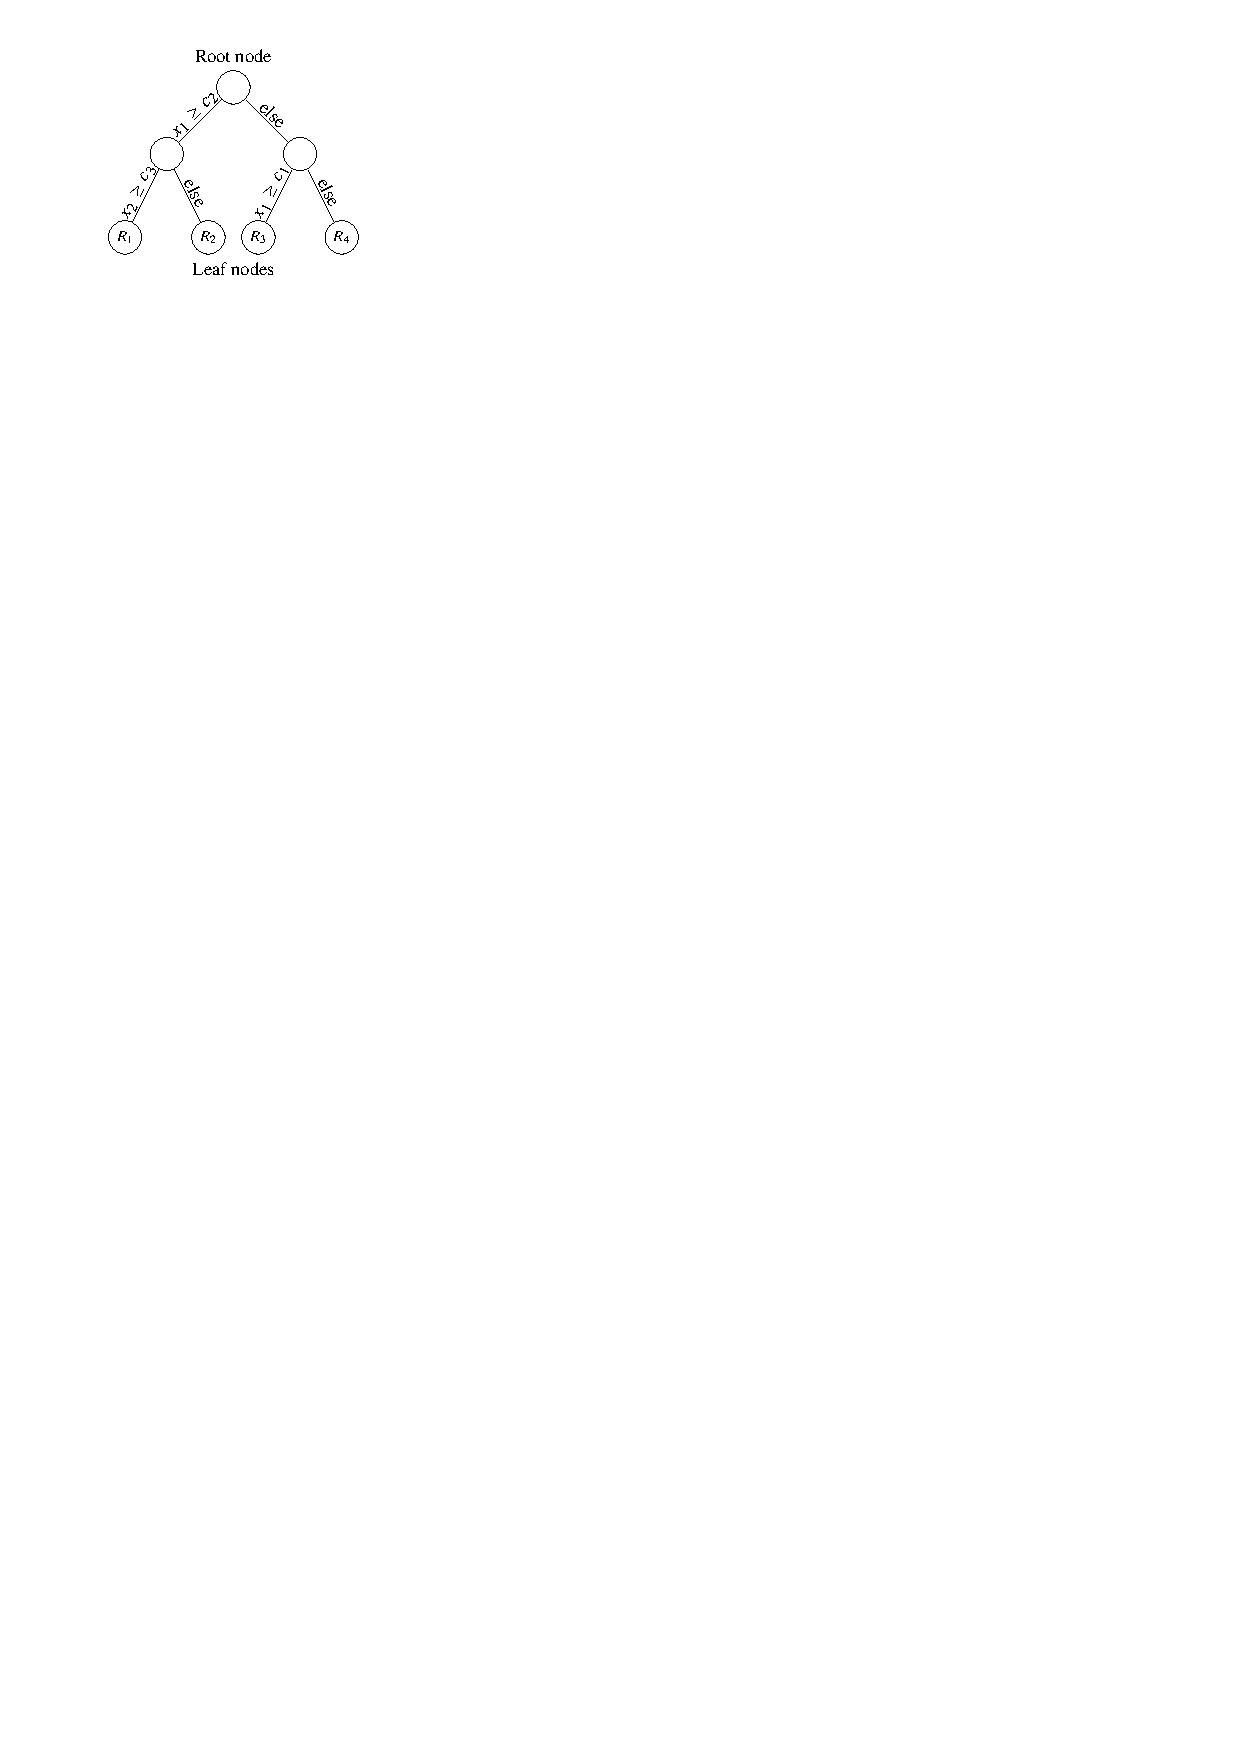
\includegraphics[scale=1.05]{ml/decision_tree}
    \caption{Binary tree structure of a decision tree.}
  \end{subfigure}\hfill%
  \begin{subfigure}[b]{0.46\textwidth}
    \centering
    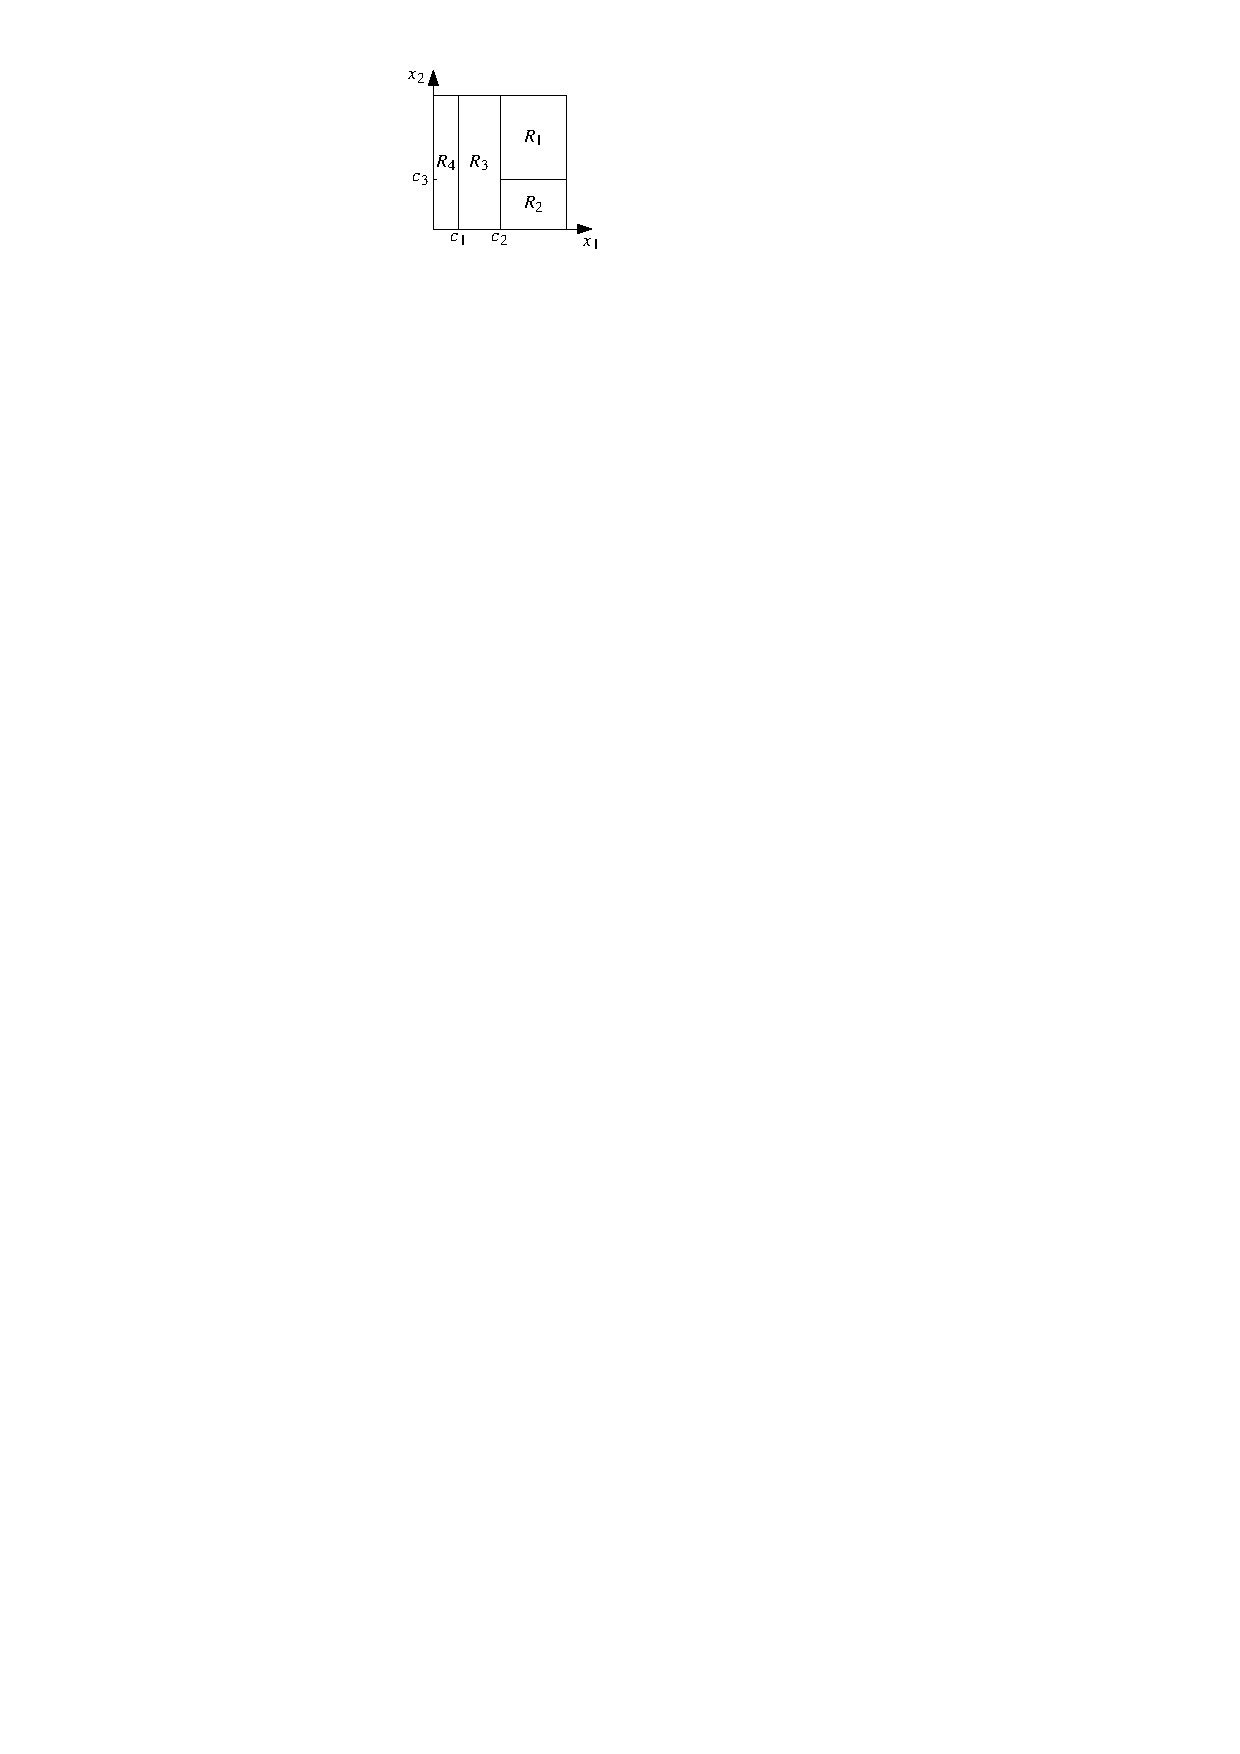
\includegraphics[scale=1.05]{ml/decision_tree_partitioning}
    \vspace*{0.7em}
    \caption{Partitioning resulting from the binary tree in (a).}
  \end{subfigure}\hfill%

  \caption{Example of a decision tree in a two-dimensional space with
    coordinates $\myvec{x} = (x_1, x_2)$. The tree has a depth of two and four
    leaf nodes that define the regions $R_1, \dots, R_4$. The figure is adapted
    from Ref.~\cite{hastie09}.}%
  \label{fig:decision_tree}
\end{figure}

Classification trees are constructed with the goal that the partitioning of the
input space yields subregions with low impurity, that is, the regions are mostly
populated by training examples of a single class. In this case, the impurity of
a tree node is quantified by the Gini index
\begin{align*}
  I_{\text{G}}(p) = 2 p (1 - p) \,\text{,}
\end{align*}
where $p$ is the proportion of examples from the positive class in a given
node~\cite{hastie09}. A \emph{greedy} strategy is adopted to grow decision trees
by performing the best possible split at every node. This split is determined by
minimising the weighted sum of Gini impurities of the resulting daughter nodes,
where impurities are weighted according to the total weight of training examples
populating a given node. In the classification case, the constants $c_j$
assigned to leaf nodes of the tree are either--depending on the algorithm
configuration--the proportion of examples from the positive class or the class
label of the majority class in a given leaf node.

Regression trees are constructed using a similar approach, however, with an
altered splitting criterion and different assigment of constants to leaf
nodes. Consider the split of a parent node into a left (L) and right (R)
daughter node. Let $(y, w)$ denote the tuple of regression target and weight of
a given training example. Moreover, let $T_{\text{L}}$ and $T_{\text{R}}$ denote
the set of $(y, w)$ for training examples populating the left and right daughter
node, respectively. The constants $c_{\text{L}}$ and $c_{\text{R}}$ assigned to
the daughter nodes are given by
\begin{align*}
  c_{\text{L}} = \frac{\sum_{(y, w) \in T_{\text{L}}} w y}{\sum_{(y, w) \in T_{\text{L}}} w} \qquad \text{and} \qquad c_{\text{R}} = \frac{\sum_{(y, w) \in T_{\text{R}}} w y}{\sum_{(y, w) \in T_{\text{R}}} w} \,\text{,}
\end{align*}
which is the weighted mean of the regression target for the training examples
populating the left and right node, respectively. The best possible split of a
node in a regression tree is chosen such that the squared error defined as
\begin{align*}
  \sum_{(y, w) \in T_{\text{L}}} w (y - c_{\text{L}})^2 + \sum_{(y, w) \in T_{\text{R}} } w (y - c_{\text{R}})^2
\end{align*}
is minimised.


\subsubsection{Boosting of Decision Trees}

The general idea of boosting is to solve a given prediction task by constructing
an additive model of the form
\begin{align*}
  F_{M}(\myvec{x}) = \sum_{m = 1}^{M} \beta_m b(\myvec{x}; \gamma_m) \,\text{,}
\end{align*}
where $\beta_m$ are coefficients and $b(\myvec{x}; \gamma_m)$ are basis
functions with parameters~$\gamma_{m}$.
















%gradient boosting~\cite{} in a binary classification setting.







is to solve a prediction task using an additive
model of the form
\begin{align*}
  F_{M} = \sum_{m = 1}^{M} \beta_m b(\myvec{x}; \gamma_m) \,\text{,}
\end{align*}
where






stagewise fashion


is a function with
parameters.







expansion with respect to some basis functions $b(\myvec{x}; )$





using an additive expansion



where




A number of boosting algorithms exist such as
\textsc{AdaBoost}~\cite{freund_shapire:adaboost,freund_shapire:adaboost2} and
the more general framework of \emph{gradient boosting}~\cite{Friedman:2001wbq}.





Boosting fits an additive expansion

\begin{align*}
  F_M(\myvec{x}) = \sum_{m = 1}^{M} \beta_m b(\myvec{x}; \gamma_{m})
\end{align*}


% construct an additive model
% \begin{align*}
%   F(x) = \sum_{m = 1}^{M} \beta_m b(x; \gamma_m) \,\text{,}
% \end{align*}
% where $b(x; \gamma_m)$

\textsc{AdaBoost}~\cite{freund_shapire:adaboost,freund_shapire:adaboost2} and
more general gradient boosting techniques that allow to minimise an arbitrary
differentiable loss function.  In this thesis, the gradient boosting
implementation of TMVA~\cite{TMVA} is used which implements the
\textsc{TreeBoost} algorithm by Friedman~\cite{Friedman:2001wbq}.

% \begin{align*}
%   F(\myvec{x}) = \sum_{m = 1}^{M} \beta_m b(\myvec{x}; \gamma_{m})
% \end{align*}

additive stagewise additive

Gradient boosting -> optimise arbitrary differentiable loss function

As a result, versatile (can do classification, regression (mean, quantile)



\textsc{TreeBoost} by Friedman~\cite{Friedman:2000,Friedman:2001wbq}




>>>>>>>>





In a binary classification setting with predictors~$\myvec{X}$ and class labels
$Y = +1$ for the positive and $Y = -1$ for the negative class,



\begin{align*}
  L(Y, F(\myvec{X})) = \log\bigl( 1 + e^{-2 Y F(\myvec{X})} \bigr)
\end{align*}






\begin{align*}
  F(\myvec{x})
  = \argmin_F \, \expect[ L(Y, F(\myvec{X})) \mid \myvec{X} = \myvec{x} ]
  = \frac{1}{2} \log\frac{
  \mathbb{P}(Y = +1 \mid \myvec{X} = \myvec{x})
  }{
  \mathbb{P}(Y = -1 \mid \myvec{X} = \myvec{x})
  }
\end{align*}





Use an additive stagewise model to approximate
\begin{align*}
  F(\myvec{X}) = \frac{1}{2} \log\left[ \frac{p(\myvec{X})}{1 - p(\myvec{X})} \right] \qquad \text{with} \qquad p(\myvec{X}) = \mathbb{P}(Y = +1 \mid \myvec{X})
\end{align*}
which is half the log-odds of the positive class.


Binary cross entropy
\begin{align*}
  L(Y, F(\myvec{X})) &=
  \begin{cases}
    - \log( p(\myvec{X}) ), & Y = +1 \\
    - \log( 1 - p(\myvec{X}) ), & Y = -1
  \end{cases} \\[0.3em]
                     &= \log\bigl( 1 + e^{-2 Y F(\myvec{X})} \bigr)
\end{align*}


The \textsc{TreeBoost} algorithm for binary classification and $M$ iterations of
boosting is described in the following. The description is based on algorithm
proposed by Friedman~\cite{Friedman:2001wbq} with few modifications as
implemented in TMVA~\cite{TMVA}:
\begin{enumerate}
  \setlength{\itemsep}{5pt}

\item Initialise $F_0(\myvec{x}) = 0$

\item For $m = 1$ to $M$:
  \begin{enumerate}
    \setlength{\itemsep}{5pt}

  \item Calculate the pseudoresiduals
    \begin{align*}
      r_i
      = - \left. \frac{\partial L(y_i, F(\myvec{x}_i))}{\partial F(\myvec{x}_i)}\right|_{F(\myvec{x}_i) = F_{m - 1}(\myvec{x}_i)}
      \overset{\text{BCE}}{=} \frac{2 y_i}{1 + \exp(2 y_i F_{m-1}(\myvec{x}_i))}
    \end{align*}
    for all training examples, where $\myvec{x}_i$ are the predictors and
    $y_i \in \{ -1, +1 \}$ the class label of the $i$-th training example,
    respectively.

  \item Using the training data, fit a regression tree to estimate the
    pseudoresiduals given the predictors~$\myvec{x}$. The prediction of the
    $m$-th regression tree is denoted by
    $h\bigl( \myvec{x}; \{c_{jm}, R_{jm}\}_{j=1}^{J_{m}} \bigr)$, where $J_{m}$
    is the number of leaf nodes, $c_{jm}$ is the prediction of the $j$-th leaf
    node, and $R_{jm}$ is the region defined by the $j$-th leaf node.

  \item The predictions of the leaf nodes of the regression tree,
    $\{c_{jm}\}_{j=1}^{J_{m}}$, are updated to minimise
    \begin{align*}
      \sum_i w_i \, L\bigl( y_i, F_{m - 1}(\myvec{x}_i)
      + h\bigl( \myvec{x}_i; \{c_{jm}, R_{jm}\}_{j=1}^{J_{m}} \bigr) \bigr)
      \,\text{,}
    \end{align*}
    which is equivalent to minimising the average loss as estimated using the
    finite sample of training data. This optimisation problem has no analytical
    minimiser. Instead, the $\{c_{jm}\}_{j=1}^{J_{m}}$ are chosen to
    approximately minimise the above criterion by performing a single step of
    Newton's method. This yields updated leaf node constants
    \begin{align*}
      c_{jm}^\prime = \frac{ \sum_i w_i r_i }{ \sum_i w_i |r_i| (2 - |r_i|)} \,\text{,}
    \end{align*}
    where the sum goes over all training examples populating the $j$-th leaf of
    the tree. This step is specific to the \textsc{TreeBoost} algorithm proposed
    by Friedman.

  \item Perform a gradient descent step by setting
    \begin{align*}
      F_m(x) = F_{m - 1}(x) + \nu \, h(\myvec{x}; \{c_{jm}^\prime, R_{jm}\}_{j=1}^{J_{m}}) \,\text{,}
    \end{align*}
    where $0 < \nu \leq 1$ is a hyperparameter of the algorithm referred to as
    the \emph{shrinkage} or \emph{learning rate}.  \todo[inline]{The shrinkage
      serves as a method of regularisation. I.e.\ by not taking he close to
      optimal step.}

  \end{enumerate}

\item The final prediction of the boosting procedure, $F_{M}(x)$, is used to
  estimate the probability $p(x) = \mathbb{P}(Y = +1 \mid x)$ according to
  \begin{align*}
    \hat{p}(x) = \frac{1}{1 + \exp(-2 F_{M}(x))} \,\text{.}
  \end{align*}
\end{enumerate}

Gradient descent in function space...


\subsection{Neural Networks}

\subsubsection{Recurrent Neural Networks}%
\label{sec:rnn}


%%% Local Variables:
%%% mode: latex
%%% TeX-master: "../../phd_thesis"
%%% End:
